\documentclass{article}

\usepackage[margin=0.5in]{geometry}
\usepackage{multicol}
\usepackage{graphicx}
\usepackage{tkz-euclide}
\usepackage{amsthm}
\usetikzlibrary{decorations.markings,arrows}
\tikzset{
    arrowMe/.style={
        postaction=decorate,
        decoration={
            markings,
            mark=at position .5 with {\arrow[thick]{#1}}
        }
    }
}

\theoremstyle{definition}
\newtheorem*{solution}{Solution}
\title{Problem-Solving Set A}
\author{}
\date{}

\begin{document}
\maketitle
\begin{multicols*}{2}
    \begin{enumerate}
        \item Five cards are lying on a table as shown.
            \begin{center}
                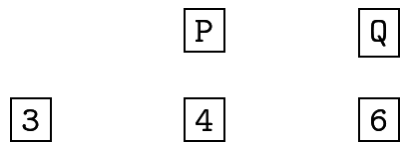
\includegraphics[scale=0.25]{5-2_cards.png}
            \end{center}
            Each card has a letter on one side and a whole number on the other side.
            Jane said, ``If a vowel is on one side of any card, then an even number is on the other side.''
            Mary showed Jane was wrong by turning over one card.
            Which card did Mary turn over?
            \begin{solution}
                For Mary to show Jane wrong, she must find a card with an odd number on one side, and a vowel on the other side.
                The only card that could possibly have this property is the card with $3$.
            \end{solution}
        \item In a magic triangle, each of the six whole numbers $10$ - $15$ is placed in one of the circles so that the sum, $S$, of the three numbers on each side of the triangle is the same.
            What is the the largest possible for $S$?
            \begin{center}
                \begin{tikzpicture}[scale=0.75]
                    \tkzDefPoint(0,0){A}
                    \tkzDefPoint(60:4){B}
                    \tkzDefPoint(4,0){C}
                    \tkzDrawPolygon(A,B,C)

                    \foreach \initpoint\finpoint\name in {A/B/D, C/B/E, C/A/F}
                    {
                        \tkzDefMidPoint(\initpoint,\finpoint)
                        \tkzGetPoint{\name}
                    }

                    \foreach \point in {A, B, C, D, E, F}
                    {
                        \tkzDrawCircle[R,fill=white](\point,0.25cm)
                    }
                \end{tikzpicture}
            \end{center}
            \begin{solution}
                To make the sum the greatest, put the three largest numbers $(13, 14, 15)$ in the corners.
                Then, balance the sides by putting the least integer $(10)$ between the greatest sum $(14 + 15)$.
                Then put the next lest integer $(11)$ between the next greatest sum $(13 + 15)$.
                Fill in the last integer $(12)$ and you can see that the sum of any three numbers on a side is (for example) $14 + 10 + 15 = 39$.
            \end{solution}
        \item Alan, Beth, Carlos, and Diana were discussing their possible grades in mathematics class this grading period.
            Alan said, ``If I get an A, then Beth will get an A.''
            Beth said, ``If I get an A, then Carlos will get an A.''
            Carlos said, ``If I get an A, then Diana will get an A.''
            All of these statements were true, but only two of the students received an A.
            Which two received A's?
            \begin{solution}
                Let's say that Alan gets an A. Well, from his statement, then Beth would also get an A.
                But from her statement, Carlos would get an A.
                And from his statement, Diana would also get an A.
                So all $4$ would get A's, but the problem said only $2$ got A's. \\
                Let's say that Beth gets an $A$.
                From her statement, we know that Carlos gets an A, and from his statement we know Diana gets an A.
                But that makes $3$, which is not $2$. \\
                If Carlos gets an A, then Diana gets an A.
            \end{solution}
        \item Let $o$ be an odd whole number and let $n$ be any whole number.
            Which of the following statements about the whole number $(o^2 + no)$ is always true?
            \begin{itemize}
                \item It is always odd.
                \item It is always even.
                \item It is even only if $n$ is even.
                \item It is odd only if $n$ is odd.
                \item It is odd only if $n$ is even.
            \end{itemize}
            \begin{solution}
                Let's say that $n$ is odd.
                If $n$ is odd, then obviously $no$ will be odd as well, since $o$ is odd, and the product of two odd numbers is odd.
                Since $o$ is odd, $o^2$ will also be odd.
                And adding two odd numbers makes an even number, so if $n$ is odd, the entire expression is even.
                Let's say that $n$ is even.
                If $n$ is even, the $no$ will be even as well, because the product of an odd and an even is even.
                $o^2$ will still be odd.
                That means that the entire expression will be odd, since the sum of an odd and an even is odd.
            \end{solution}
        \item Using only the paths and the directions shown, how many different routes are there from $M$ to $N$.
            \begin{center}
                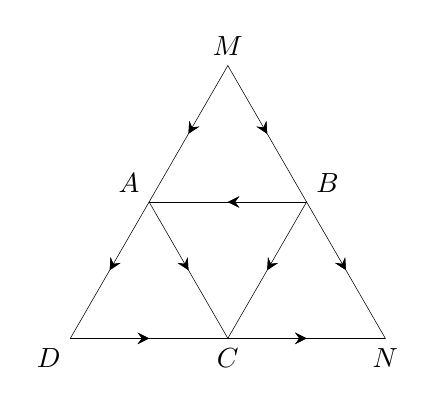
\begin{tikzpicture}
                    \tkzDefPoint(0,0){D}
                    \tkzDefPoint(60:4){M}
                    \tkzDefPoint(4,0){N}

                    \foreach \initpoint\finpoint\name in {D/M/A, M/N/B, D/N/C}
                    {
                        \tkzDefMidPoint(\initpoint,\finpoint)
                        \tkzGetPoint{\name}
                    }

                    \tkzLabelPoint[below left](D){$D$}
                    \tkzLabelPoint[above](M){$M$}
                    \tkzLabelPoint(N){$N$}
                    \tkzLabelPoint[above left](A){$A$}
                    \tkzLabelPoint[above right](B){$B$}
                    \tkzLabelPoint[below](C){$C$}

                    \tkzDrawSegments[arrowMe=stealth](M,A M,B B,A A,C B,C A,D D,C C,N B,N)
                \end{tikzpicture}
            \end{center}
            \begin{solution}
                There is $1$ way to get from $C$ to $N$.
                There is only one way to get from $D$ to $N$, which is $DCN$.
                Since $A$ can only go to $C$ or $D$, which each only have $1$ way to get to $N$ each, there are $1 + 1 = 2$ ways to get from $A$ to $N$. \\
                Since $B$ can only go to $A$, $C$ or $N$, and $A$ only has $2$ ways to get to $N$, $C$ only has $1$ way and to get from $B$ to $N$ is only $1$ way, there are $2 + 1 + 1 = 4$ ways to get from $B$ to $N$. \\
                $M$ can only go to either $B$ or $A$, $A$ has $2$ ways, and $B$ has $4$ ways, so $M$ has $4 + 2 = 6$ ways to get to $N$.
            \end{solution}
        \end{enumerate}
\end{multicols*}
\end{document}